
\section{Trattamento riabilitativo della coxartrosi}


\subsection{COXARTROSI}



\emph{L'artrosi degenerativa dell'anca provoca una limitazione del
movimento femorale.}

\emph{Ne consegue un importante impatto sulla funzione del cingolo
pelvico e sul rachide lombare, poiché entrambi tentano di compensare la
perdita di movimento a livello dell'anca.}

\paragraph{Valutazione}


\emph{All'\textbf{ispezione} è evidente, soprattutto nelle forme più
avanzate, un atteggiamento in adduzione, flessione e rotazione esterna, più raramente interna.}

\emph{Alla \textbf{palpazione} possono riscontrarsi punti dolorosi
dell'articolazione.}

\emph{Alla \textbf{valutazione dei singoli movimenti} si ha una
riduzione della flessione e, in misura maggiore e più precocemente,
dell'abduzione, dell'intra ed extrarotazione e dell'estensione (il
paziente fa fatica ad infilare le calze, a calzare le scarpe, a scendere o salire le scale). Negli
stadi iniziali solo attività di maggior impegno articolare, come quelle sportive, determinano un aggravamento
della situazione. Instaurata la malattia si avranno i \textbf{risultati
a livello radiologico:} riduzione dell'interlinea articolare; gli osteofiti costituiscono
un segno radiologico precoce e possono rilevarsi fenomeni di
osteosclerosi e rarefazione a stampo (geodi).}

\emph{L'\textbf{evoluzione} è lenta ed inesorabile e conduce ad un
aggravamento progressivo con limitazione dei movimenti fino all'anchilosi.}

\emph{La degenerazione artrosica può avere molteplici cause, di
particolare importanza è l'aspetto biomeccanico: una disfunzione dei
sistemi articolare e neuromuscolare può dar luogo ad una cattiva
distribuzione dei carichi, favorendo lo sviluppo di coxartrosi.}
\paragraph{Obiettivi}



\begin{itemize}
\item
  \emph{Riduzione del dolore e della reattività articolare}
\item
  
  \emph{Aumento dell'ampiezza articolare}
  
\item
  \emph{Miglioramento della stabilità articolare }
\end{itemize}
\paragraph{Principali strategie di intervento terapeutico}

\begin{itemize}
\item 
\emph{- Tecniche articolari: trazione, traslazione, roll, swing,
movimenti osteocinematici}
\item 
\emph{- Tecniche legamentose/tendinee: mobilizzazioni, trazioni}
\item 
\emph{- Tecniche muscolari: stretching, contrazioni isotoniche ed
isometriche}
\item 
\emph{- Tecniche neuro dinamiche: sollevamento dell'arto inferiore
esteso, propriocettiva}
\item 
\emph{- Combinazione di 2 o più tecniche}
\item 
\emph{- Massoterapia}

\item 
\emph{- Termoterapia, elettroterapia, ultrasuonoterapia, laserterapia,
ortesi}
\end{itemize}
\section{Trattamento riabilitativo pre-intervento chirurgico all'anca}

\emph{L'artroprotesi totale di anca prevede un percorso riabilitativo
ben definito finalizzato a restituire la funzionalità dell'articolazione
e possibilmente a migliorare quella precedente all'intervento.}

\emph{Studi recenti hanno evidenziato come un trattamento pre-chirurgico
dia le migliori garanzie post-intervento dal punto di vista della
performance muscolare e motoria; ciò soprattutto in vista della ripresa
dell'attività lavorativa e sociale del soggetto.}

\emph{\textbf{L'obiettivo del trattamento pre-chirurgico} è far sì che
il paziente si abitui sin da subito a svolgere esercizi per il recupero
del tonotrofismo muscolare; in questo modo si presenterà all'intervento
con una buona condizione muscolare e ciò accelererà i tempi di
recupero.}

\emph{Inoltre la riabilitazione pre-chirurgica educa il paziente
all'utilizzo degli arti brachiali e alla gestione del carico.}

\emph{Nella \emph{fase pre-operatoria} il fisiatra deve}


\begin{itemize}
\item
  
  \emph{valutare la sintomatologia dolorosa}
  
\item
  
  \emph{valutare la capacità di deambulare con o senza ausili}
  
\item
  
  \emph{valutare se dolore e impedimento possono causare disabilità e
  peggiorare gli atti della vita quotidiana.}
  
\end{itemize}



\emph{Esiste a questo scopo la Scala di valutazione \textbf{WOMAC}, che
appunto valuta la sintomatologia dolorosa, l'arco di movimento
dell'articolazione e la capacità del soggetto di attendere agli atti
della vita quotidiana. Essa inoltre permette di monitorare l'esito
dell'intervento chirurgico e di quello riabilitativo. Riassumendo, nella
fase pre-operatoria il paziente va istruito su: esercizi preintervento,
consigli sulle corrette posture da assumere nel periodo di ricovero, uso
di ausili e calzature adeguate per il percorso riabilitativo previsto.
Inoltre, in base alle condizioni cliniche preintervento del paziente si
deciderà la sede del trattamento riabilitativo. Se il soggetto è giovane
e compliante e necessita di un rapido recupero va diretto verso un
percorso ambulatoriale; un altro soggetto anziano e con comorbilità va
invece riabilitato nelle strutture apposite o a casa.}

\emph{Dal punto di vista riabilitativo possiamo citare: }

\begin{enumerate}
\item 
\textit{un trattamento con mezzi fisici:}
\item
  \emph{chinesiterapia}
\item
  \emph{condroprotezione}
\end{enumerate}

\subsection{Campi elettromagnetici pulsati}

La magnetoterapia è utilizzata da molto tempo in ambito ortopedico per
stimolare la riparazione ossea e quindi favorire la formazione del callo
osseo (\textbf{effetto osteogenetico}).

Si utilizzano \emph{campi magnetici pulsati} perché la pulsazione
permette di lavorare con frequenze e potenze che possono arrivare ad un
picco sufficiente a dare l'effetto sulla stimolazione osteoblastica. Poi
si regredisce e si ripartire nuovamente.

L'onda è formata da

\begin{itemize}
\item
  un'area di tensione
\item
  un'area di compressione.
\end{itemize}


Questo effetto è molto importante specialmente in quei casi dove c'è una
fase iniziale di riduzione della rima articolare; infatti nelle fasi più
avanzate, con degli osteofiti, questo tipo di percorso ha poca
efficacia.


\subsection{Kinesiterapia}

I benefici principali della kinesiterapia sono:

\begin{enumerate}
\def\labelenumi{\arabic{enumi}.}
\item
  mantenimento dell'escursione articolare
\item
  mantenimento della stabilità articolare con esercizi di potenziamento
\item
  prevenzione ipotonie/ipotrofie articolari
\end{enumerate}

Riguardo il \textbf{mantenimento dell'escursione articolare,} la
kinesiterapia ha un ruolo importante nella prevenzione della limitazione
funzionale legata alla \emph{patologia artrosica degenerativa}: mediante
un esercizio fisico a basso impatto e a bassa energia si può avere un
effetto importante su:

\begin{itemize}
\item ~
 \textit{rimineralizzazione
  ossea}
\item
  \textbf{attività del muscolo}, che si mantiene allenato e aiuta
  l'articolazione a non irrigidirsi, evitando quei gradi di limitazione
  articolare che portano poi alla sintomatologia dolorosa
\end{itemize}

Soggetti in cui può essere utile questo tipo di trattamento sono ad
esempio: soggetti anziani, soggetti con displasia congenita dell'anca,
pazienti nei quali è importante mantenere funzioni adeguate.

\begin{itemize}
\item
  In passato esisteva un lettino particolare costituito da una grata
  montata a baldacchino ad una altezza di 1,60 m sopra il lettino
  stesso, che serviva ad agganciare delle carrucole imbragate all'arto e
  fare in modo che il soggetto facesse \textbf{automobilizzazione
  dell'articolazione} con movimenti di flesso-estensione e
  adduzione-abduzione dell'arto.
\item
  Con il tempo poi si passò a sistemi più complessi dove questa
  carrucola si poteva collegare ad un leggero peso (che poteva via via
  aumentare) ed il soggetto doveva sollevare l'arto contro una debole
  resistenza. In alternativa si usava una banda elastica.
\end{itemize}

\subsection{Idrokinesiterapia}


Consiste in \textbf{trattamenti terapeutici in acqua} a T tra 28\textsuperscript{o}-30\textsuperscript{o}C.


Sfruttando il galleggiamento si riduce la forza peso sull'articolazione
e si compiono movimenti

che al di fuori dall'acqua sarebbero difficili, se non impossibili.

Si aumenta progressivamente il carico riducendo il peso di appoggio.

Effetti terapeutici:

\begin{itemize}
\item
  
  analgesia
  
\item
  
  decontrazione
  
\item
  
  rilassamento
  
\item
  
  aumento escursione articolare
  
\item
  
  miglioramento della circolazione
  
\item
  
  miglioramento stato della cute
  
\item
  
  effetti psicologici
  
\end{itemize}

In acqua si possono anche fare esercizi sfruttando la stimolazione
dell'acqua dal punto di visto propriocettivo ed esterocettivo: si deve
infatti mantenere l'equilibrio e questo è possibile solo se si mantiene
una posizione stabile con muscolatura attiva.

Se poi ci avvaliamo dell'utilizzo di sistemi che ci permettono di
aumentare la spinta idrodinamica (galleggianti) abbiamo la possibilità
di far eseguire al nostro soggetto un movimento passivo puro.

\subsection{Elettroterapia con onde rettangolari}

Terapia alternativa all'idrokinesi, oggi stranamente non più utilizzata
nonostante la sua notevole efficacia.


Il sistema attuale prevede il lavoro sul paziente con la \textbf{terapia
manuale}:


\begin{itemize}
\item
  
  la \emph{fisioterapia} per ridurre la contrattura muscolare
  
\item
  
  la \emph{kinesiterapia} per lavorare sull'articolarità
  
\item
  
  la \emph{contrazione muscolare contro resistenza} per il rinforzo
  muscolare. È tutto condizionato dal terapista.
  
\end{itemize}

Con l'elettroterapia, invece, il paziente è sollecitato ad eseguire il
movimento in maniera autonoma o auto-assistita.


L'elettroterapia di rinforzo muscolare si distingue in due tipologie a
seconda che agisca su:


\begin{itemize}
\item
  muscolo normalmente innervato
\item
  muscolo parzialmente innervato.
\end{itemize}

\begin{figure}[!ht]
\centering
	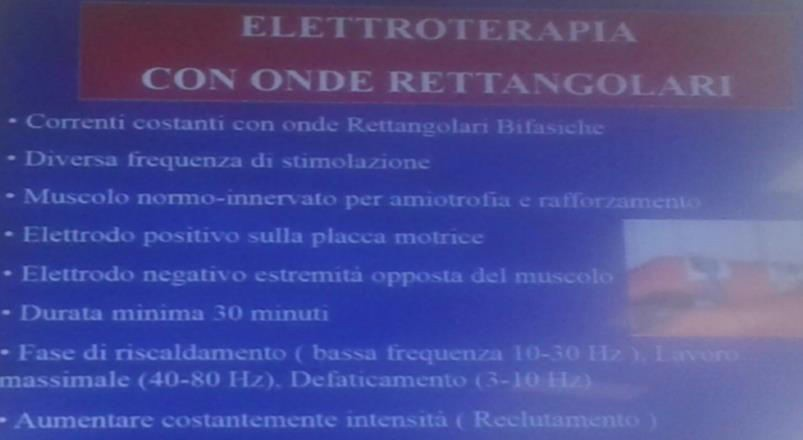
\includegraphics[width=0.7\textwidth]{031/image1.jpeg}
\end{figure}


Si tratta di \textbf{onde rettangolari bifasiche} che hanno un effetto
di potenziamento muscolare in un muscolo ipotrofico normalmente
innervato.


L'\emph{elettrodo positivo} è posizionato nella zona dove
presumibilmente si trova la \emph{placca motrice}, zona dove il muscolo
dovrebbe essere maggiormente rappresentato (per il quadricipite circa a
metà della coscia).

Per identificare la placca motrice in maniera specifica occorre
utilizzare un sistema elettromiografico particolare: consiste in
\textbf{elettrodi a schiera}, posizionati e collegati ad un sistema che
permette di vedere la contrazione del muscolo ed il comportamento
dell'onda di contrazione.

Quando quest'onda raggiunge il plateau e cambia direzione (s'inverte),
lì sicuramente è presente la placca motrice.

L'\emph{elettrodo negativo} è posizionato all'\emph{estremità opposta}
del muscolo.

La seduta standard di terapia è di 30 minuti.

Lo stimolo applicato deve essere gradualmente aumentato perché ci sarà
con il tempo un certo adattamento del paziente allo stesso.

Gli apparecchi per l'elettroterapia possono avere più uscite, le quali
possono essere posizionate su più gruppi muscolari.

Se si tratta il quadricipite, per agire su tutta la componente si
dovrebbero stimolare anche i vasti (vasto laterale e vasto mediale), e
gli ischiocrurali.


Così facendo \textbf{si stimolano agonisti ed antagonisti} per mantenere
il normale rapporto muscolare senza creare squilibri muscolari.


\subsection{Terapia a trasferimento energetico per contatto capacitivo e resistivo}

Nelle fasi di riacutizzazione del processo artrosico (in fase subacuta)
si utilizza la terapia a trasferimento energetico per contatto
capacitivo e resistivo, o \textbf{diatermia}.

È un sistema di \textbf{ipertermia endogena} con cui si produce calore
in profondità, quindi utile per agire su articolazioni posizionate in
profondità.

L'effetto è di \textbf{attivazione} nella zona trattata con
\emph{aumento del flusso ematico} e buona \emph{azione}
\emph{antinfiammatoria}.

Si possono usare due sistemi di lavoro:

\begin{itemize}
\item
  \emph{Sistema capacitivo}: trattamento di tessuti molli, tendini e
  fasce.
\item
  \emph{Sistema resistivo}: per lavorare in profondità sulle
  articolazioni.
\end{itemize}

Un trattamento ha durata di 30 minuti, con sistema misto
capacitivo-resistivo (di durata diversificata di ciascun sistema).
\begin{figure}[!ht]
\centering
	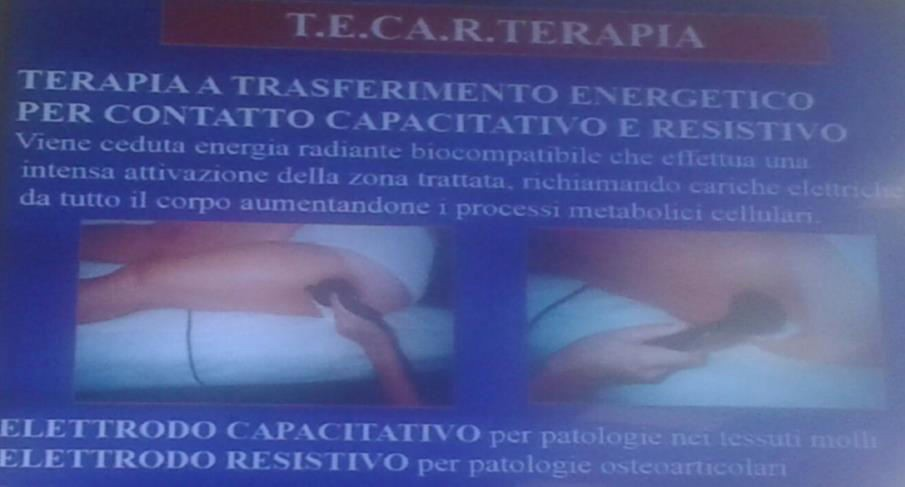
\includegraphics[width=0.7\textwidth]{031/image2.jpeg}
\end{figure}


\emph{Altra terapia utilizzata nelle patologie artrosiche in generale è la \textbf{laserterapia} grazie al suo effetto anitinfiammatorio antalgico e biostimolante e grazie al fatto che
adesso esistano apparecchi con delle potenze abbastanza elevate come
richiede un'articolazione ben protetta come è quella del ginocchio.}

\paragraph{LA CONDROPROTEZIONE}


\emph{La terapia farmacologica dell'artrosi si basa su: - controllo del
sintomo :FANS, analgesici}

\begin{itemize}
\item
  \emph{controllo danno strutturale : CONDROPROTETTORI}
\end{itemize}

\emph{La patogenesi dell'osteoartrosi prevede l'infiammazione della
membrana sinoviale con degenerazione cartilaginea. I programmi di cura
prevedono diversi tipi di farmaci:}

\begin{itemize}
\item
  \emph{\textbf{Fast-Acting Drug for OsteoArthritis}: Analgesici, FANS,
  Corticosteroidi IntraArticolari}
\item
  \emph{\textbf{Slow-Acting Drug for OsteoArthritis:} Condroitinsolfato,
  Acido ialuronico IA, Glucosamina solfato}
\item
  \textbf{Disease Modifying Drug for OsteoArthritis}: Glucosamina
  solfato, Acido ialuronico IA
\end{itemize}

Caratteristiche del condroprotettore ideale:

\begin{itemize}
\item
  
  inibizione dei processi degradativi della cartilagine
  
\item
  
  conservazione del metabolismo condrocitario
  
\item
  
  mantenimento delle caratteristiche reologiche del liquido sinoviale
  
\item
  stimolazione della sintesi condrocitaria e sinoviocitaria di acido
  ialuronico, proteoglicani e collagene \textbf{L'ACIDO IALURONICO} è il
  principale responsabile delle caratteristiche viscoelastiche del
  liquido sinoviale, è fisiologicamente sintetizzato dai sinoviociti B,
  garantisce l'attività di filtro della membrana sinoviale, il bilancio
  idrico tissutale, le interazioni steriche e la lubrificazione.
  
  \emph{Nell'osteoartrosi sono diminuiti la concentrazione ed il peso
molecolare dell'acido ialuronico a causa di diluizione secondaria al
versamento, diminuzione della sintesi, degradazione dello stesso A I nel
liquido sinoviale}

\end{itemize}




\emph{Il concetto di \textbf{VISCOSUPPLEMENTAZIONE} è basato
sull'ipotesi che l'iniezione intra-articolare di AI può aiutare a ristabilire la viscoelasticità del liquido
sinoviale, migliorando la funzionalità articolare e riducendo il
dolore.}

\paragraph{EFFETTI BIOLOCICI DELL'ACIDO IALURONICO}
\subparagraph{Sulla matrice extracellulare:}


\begin{itemize}
\item
  
  \emph{Riduzione rilascio PG dalla matrice cartilaginea}
  
\item
  
  \emph{Aumentata sintesi di condroitinsolfato}
  
\item
  
  \emph{Aumentata sintesi PG in presenza di IL-1$alpha$}
  
\end{itemize}

\subparagraph{Sulla cartilagine}


\begin{itemize}
\item
  
  \emph{Soppressione degenerazione cartilaginea}
  
\item
  
  \emph{Miglioramento strato superficiale cartilagineo e riduzione
  infiammazione sinoviale}
  
\item
  
  \emph{Aumento densità e miglioramento morfologia condrociti}
  
\end{itemize}
\subparagraph{Sui mediatori dell'infiammazione}

\begin{itemize}
\item
  
  \emph{riduzione livelli PGE2 nel liquido sinoviale}
  
\item
  
  \emph{riduzione espressione IL-1$alpha$} e stromelisina e produzione NO
  
\item
  
  soppressione produzione TNF $alpha$
  
\end{itemize}
\subparagraph{Sulle cellule
immunitarie}


\begin{itemize}
\item
  
  riduzione attivazione e migrazione PMN
  
\item
  
  soppressione aggregazione e adesione neutrofila
  
\end{itemize}

Di conseguenza l'acido ialuronico stimola i processi riparativi e induce
una significativa riduzione dell'infiammazione articolare.

Durata degli effetti ed efficacia del trattamento ripetuto:
miglioramento sintomatico di lunga durata dopo 2-5 settimane, nuovo ciclo di trattamento alla ricomparsa della
sintomatologia dolorosa (\textgreater{}6mesi).

\paragraph{GLUCOSAMINA SOLFATO}


E' un normale costituente dei glicosamminoglicani e dei proteoglicani
presenti nel liquido sinoviale e nella matrice cartilaginea. Ha:

\begin{itemize}
\item
  EFFETTI ANABOLICI: aumenta la sintesi di proteoglicani
\item
  EFFETTI ANTICATABOLICI: riduce l'attività della collagenasi
  \item
    \emph{PROPRIETA' ANTINFIAMMATORIE: inibisce il rilascio di enzimi
    proteolitici, gli enzimi lisosomi ali, la sintesi di ossido nitrico inducibile}
  \end{itemize}



\paragraph{CONDROITIN SOLFATO}



\begin{itemize}
\item
  
  \emph{stimolazione sintesi pgs (1,2), aggrecani e acido ialuronico ad
  alto p.m. (3,4)}
  
\item
  
  \emph{inibizione attivita' collagenolitica}
  
\item
  
  \emph{inibizione effetti IL-1 su sintesi pgs, collagene di tipo II,
  PGE2 ed NO}
  
\item
  
  \emph{riduzione apoptosi condrocitaria indotta dall'no}
  
\item
  
  \emph{protezione in modelli animali dall'osteoartrosi}
  
\item
  
  \emph{effetto antiflogistico}
  
\end{itemize}

\subsection{Cryoultrasound}


Trattamento utilizzabile in \emph{fase acuta}, da associare ad adeguata
terapia farmacologica (analgesica e antinfiammatoria).

L'ultrasuono a freddo, o cryoultrasound, permette di utilizzare
contemporaneamente la terapia con il calore e la terapia con il freddo.


\begin{itemize}
\item
  La terapia con il \textbf{freddo} serve in caso di infiammazione
  locale a dare un effetto di vasocostrizione
\item
  In più l'apparecchio crea un cono di raffreddamento attraverso il
  quale passa la terapia con il \textbf{calore}, cioè l'onda
  ultrasonora, che crea l'effetto di riscaldamento.
\end{itemize}


Il manipolo dell'apparecchio raggiunge temperature di -10\textsuperscript{o}C, per questo
va continuamente mosso (mai lasciato fermo!) ed utilizzato solo da
personale qualificato in modalità pulsata.

Raffreddando la zona articolare interessata, si possono così utilizzare
delle potenze alte ed arrivare a livello dell'articolazione coxofemorale
senza ustionare il paziente con temperature che risulterebbero troppo
elevate.

Si possono istruire i pazienti a svolgere a domicilio alcuni esercizi
per arrivare all'intervento chirurgico in maniera adeguata.

\section{Trattamento riabilitativo della coxartrosi: programma domiciliare}

\subsection{Esercizi di stretching}


Riguardano i muscoli:


\begin{itemize}
\item
  glutei
\item
  ischiocrurale
\item
  quadricipite
\end{itemize}


Il paziente è in decubito: porta l'arto controlaterale in posizione di
ginocchio flesso a 90\textsuperscript{o} e mantiene la posizione.

In questo modo si ha un allungamento di:


\begin{itemize}
\item
  catena posteriore
\item
  quadricipite
\item
  adduttore e abduttore dell'anca
\item
  tensore della fascia lata, ottimo stabilizzatore laterale dell'arto
  inferiore e dell'anca.
\end{itemize}

\subsection{Esercizi di rinforzo muscolare}


Il movimento con cyclette è ottimale, perché permette di lavorare


\begin{itemize}
\item
  sull'angolo della gamba tramite regolazione dell'altezza del sellino
\item
  con le resistenze
\end{itemize}

\subsection{Esercizi per il mantenimento del R.O.M.}


Consiste nel mantenere l'arto in movimento, in modo da migliorare o
mantenere il Range Of Motion, cioè la flessibilità articolare.


\section{Intervento di potesizzazione}

Quando il dolore non è più tollerabile si arriva alla protesi di anca,
che risolve la sintomatologia dolorosa e la limitazione legata a questa
sintomatologia.
\begin{figure}[!ht]
\centering
	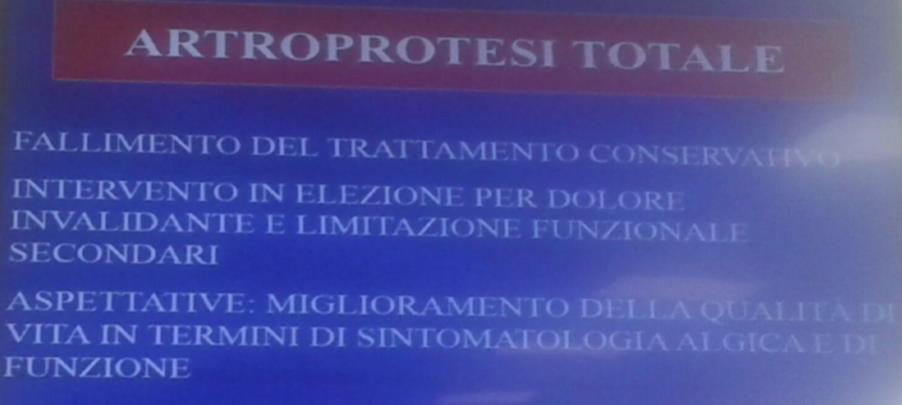
\includegraphics[width=0.5\textwidth]{031/image3.jpeg}
\end{figure}


È stato elaborato un panel europeo, dove è stato definito che il
\textbf{miglioramento della qualità di vita} di un paziente con
coxartrosi lo si ottiene sulla base di particolari situazioni favorenti
il recupero, tra cui la situazione \textbf{pre-intervento chirurgico}.


\subsection{Perché preparare il soggetto all'intervento?}


Se il soggetto è preparato dal punto di vista clinico, muscolare e
articolare:


\begin{itemize}
\item
  supererà l'intervento in maniera ottimale
\item
  si ridurrà il dolore
\item
  i tempi di recupero post-chirurgici saranno ridotti.
\end{itemize}


Il paziente può arrivare ad avere:


\begin{itemize}
\item
  la massima escursione articolare
\item
  la massima deambulazione possibile con il corretto sistema del passo
\item
  un adeguato tono muscolare per mantenere la stabilizzazione
\end{itemize}

\section{Trattamento riabilitativo post-operatorio}

\emph{Il trattamento post-intervento deve}


\begin{itemize}
\item
  
  \emph{prevenire i danni secondari all'immobilità}
  
\item
  
  \emph{agire sul dolore}
  
\item
  
  \emph{recuperare il tonotrofismo muscolare}
  
\item
  \emph{recuperare il corretto schema del passo, perché questi pazienti
  già in partenza ce l'hanno alterato. Il soggetto presenta infatti un'
  ipotonotrofia muscolare importante, soprattutto riguardante i muscoli
  glutei e ischio-crurali, quadricipite, tensore della fascia lata,
  adduttori e abduttori di anca che stabilizzano l'articolazione.}
\end{itemize}


Costituito da:


\begin{itemize}
\item
  \emph{Fase acuta}: i primi 5 giorni immediatamente successivi
  all'intervento (considerando l'intervento al giorno 1), secondo le indicazioni della regione Emilia
Romagna.
\item
  \emph{Fase post-acuta} Crioterapia intermittente (20 min di applicazione -- 10 min di
intervallo) Terapia antalgica (non necessariamente utilizzata).
\end{itemize}
Secondo la società ortopedica americana il trattamento riabilitativo
post-chirurgico nelle protesizzazioni deve essere iniziato \textbf{il
più precocemente possibile}, cioè immediatamente dopo l'intervento
chirurgico.

A Parma si inizia il trattamento riabilitativo il giorno 2 (giorno dopo
l'intervento).


\subsection{FASE ACUTA}


\paragraph{FASE DI MASSIMA PROTEZIONE (4-7 GIORNI)}


\emph{In questa fase è necessario:}
\begin{itemize}
\item 
\emph{- prevenire la dislocazione o la sublussazione, le complicanze
polmonari;}
\item
  
  \emph{raggiungere l'indipendenza nei trasferimenti prima della
  dimissione;}
  
\item
  
  \emph{mantenere la forza degli arti} superiori e dell'arto inferiore
  sano con esercizi attivi;
  
\item
  
  mantenere la mobilità dell'arto operato con esercizi di mobilizzazione
  passiva, in flessione, abduzione, rotazioni non controindicate dal tipo di accesso chirurgico;
  
\item
  
  prevenire una contrattura in flessione ponendo l'arto sano in massima
  flessione e lasciando rilassato l'arto operato, allungando i flessori dell'anca.
  
\end{itemize}




\subparagraph{I\textsuperscript{o} Giorno:}

\begin{itemize}
\item
  Applicazione di \emph{Impulsus Sistem}, utilizzato per la prevenzione
  delle tromboembolie.
\item
  Posizionamento del paziente \emph{seduto}, meglio con le gambe fuori
  dal letto.
\item
  \emph{Mobilizzazione attiva} dell'anca e del ginocchio
  (flesso-estensione), prima dell'arto sano, poi lentamente anche
  dell'arto che ha subito l'intervento.
\end{itemize}


\emph{Secondo la scuola americana, il paziente va messo in carico dopo
24 h dall'intervento, questo grazie agli effetti della terapia antalgica
infusiva; in Italia si è più cauti, ed il paziente viene verticalizzato
in terza giornata. Questo perchè in primis vanno monitorate le
complicanze vascolari dell'intervento: è vero che il paziente assume
anticoagulanti e subisce un input-system finalizzato alla ginnastica
vascolare, ma gli imprevisti non vanno sottovalutati. Il paziente poi ha
un catetere per il drenaggio dell'articolazione, e questo gli impedisce
di deambulare (NB nelle protesi d'anca non si usa praticamente
più,mentre si usa per quelle di ginocchio).}

\subparagraph{II\textsuperscript{o} Giorno:}

\begin{itemize}
\item
  Posizionamento del paziente seduto \emph{in poltrona}.
\item
  \emph{Mobilizzazione continua passiva}.

Nelle protesi di ginocchio si utilizzano i \textbf{Kitec}, apparecchi
per mobilizzazione attiva passiva.

Non ci sono evidenze in letteratura che la mobilitazione attiva passiva
sia più efficace della mobilitazione passiva fatta dal terapista, ma dà
sicuramente vantaggi in quanto


\begin{itemize}
\item
  non ha bisogno di personale dedicato
\item
  il paziente può usufruire della mobilitazione per più tempo rispetto
  al tempo di esecuzione da parte di un terapista
\item
  si può aumentare l'angolo di mobilizzazione e la velocità di
  esecuzione del movimento.
\end{itemize}

\item
  \emph{Rimozione drenaggi} (l'accesso anteriore, il cui drenaggio si
  rimuove subito, garantisce un recupero più veloce rispetto all'accesso
  laterale).
\end{itemize}
\subparagraph{III\textsuperscript{o} Giorno:}


\begin{itemize}
\item
  Recupero dell'\emph{ortostatismo}.
\item
  \emph{Deambulazione con carico sfiorante} mediante deambulatore con
  appoggio ascellare (si può fare già in seconda giornata).
\end{itemize}

\subparagraph{IV\textsuperscript{o} Giorno:}


\begin{itemize}
\item
  Deambulazione con deambulatore ad appoggio ascellare. Si dovrebbe già
  iniziare a lasciare il deambulatore ed usare i \emph{bastoni
  canadesi}.
\end{itemize}
\subparagraph{V\textsuperscript{o} Giorno:}


\begin{itemize}
\item
  \emph{Addestramento al cammino a 3 Tempi} (cammino iniziale:
  ``passo-bastone-passo'') con l'ausilio di bastoni ad appoggio antibrachiale (detti `bastoni
canadesi').
\item
  
  Successivamente si passa ad un \emph{cammino a 4 Tempi}
  (``bastone-passo-bastone- passo'').
  
\end{itemize}

Dove possibile, si può usare una piccola scala a tre gradini per far
esercitare il paziente a fare le scale con il bastone, in modo da
acquisire maggiore praticità.

\subparagraph{DIMISSIONE}


La dimissione dovrebbe avvenire, secondo le linee guida internazionali e
regionali, in V\textsuperscript{o} giornata.

Al momento della dimissione, il paziente dovrebbe saper sfruttare al
meglio i bastoni canadesi.

Se il paziente ha fatto un \textbf{percorso pre-operatorio} ed è in
condizioni adeguate, non avrebbe necessità di passare in una struttura
riabilitativa, poiché sarebbe già adeguatamente istruito a muoversi
autonomamente a casa.

Si effettuano quindi solo \emph{controlli periodici}.

Se così non fosse, si effettua un ricovero in \textbf{struttura
riabilitativa} o un trattamento in day- hospital/regime ambulatoriale.

\emph{Una volta dimessi, i pazienti possono essere inviati a domicilio o
in una struttura pubblica o privata per il programma riabilitativo; qui
svolgeranno un trattamento estensivo di 1 ora al giorno, oppure
intensivo di 2 ore al giorno con personale dedicato (cosa non possibile
in un reparto di ortopedia).}

\emph{Il setting riabilitativo dipende dalle condizioni del paziente e
dalla compliance dei familiari, oltre che dall'assenza di barriere
architettoniche a domicilio. A questo scopo il servizio territoriale
invia un terapista a domicilio che, in 5 sedute, istruirà il paziente e
i familiari su come usare il deambulatore e i bastoni canadesi
antibrachiali. Spesso infatti il paziente esce dall'ospedale usando
ancora il deambulatore ad appoggio ascellare, e la figura del terapista
a domicilio diventa quindi essenziale.}

\begin{figure}[!ht]
\centering
	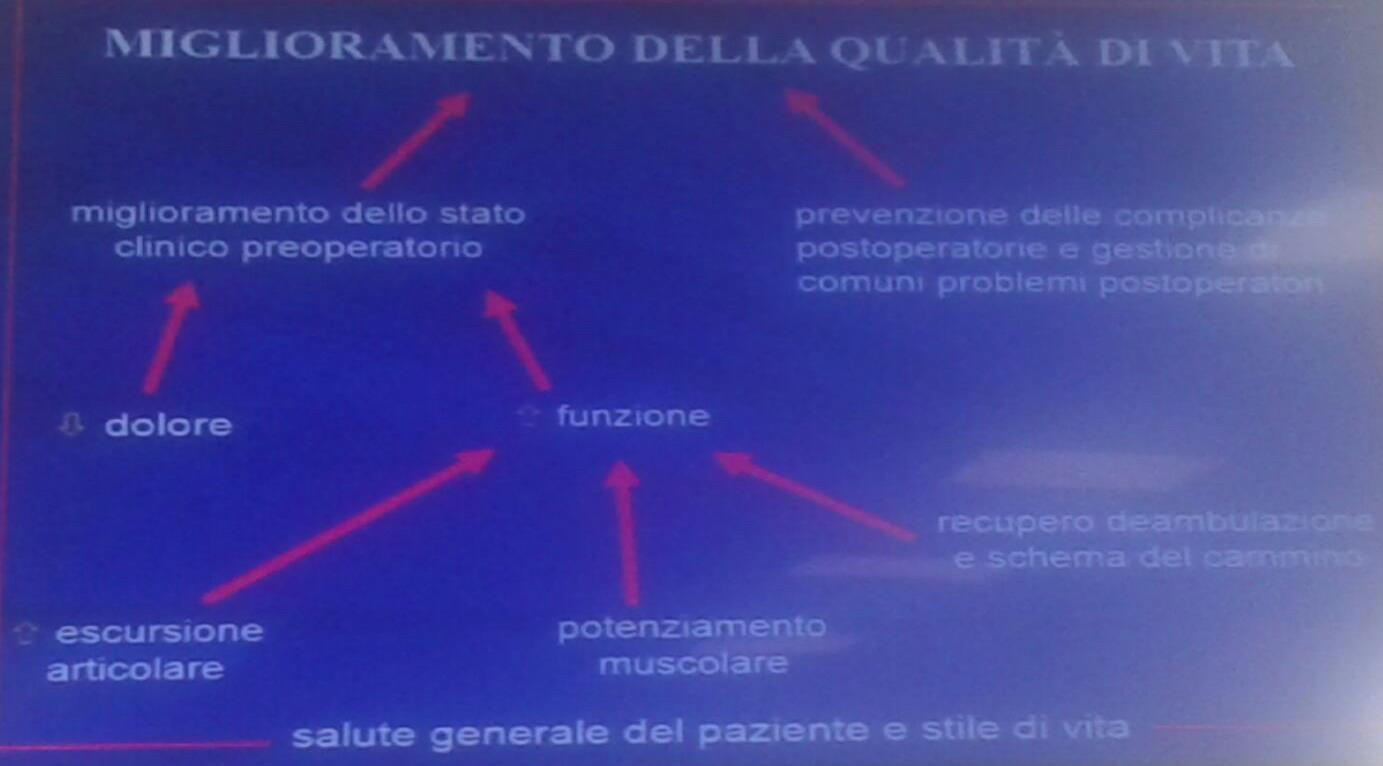
\includegraphics[width=0.7\textwidth]{031/image4.jpeg}
\end{figure}


\paragraph{FASE DI MODERATA E MINIMA PROTEZIONE (8 giorni/6-12 settimane)}


\emph{È necessario:}

\begin{itemize}
\item
  \emph{recuperare la forza, la resistenza ed il movimento articolare
  dell'arto operato con:}

\item
  
  \emph{Mobilizzazione passiva seguendo la corretta artrocinematica
  dell'anca}
  
\item
  
  \emph{Flesso estensione di anca e ginocchio strisciando il tallone sul
  lettino}
  
\item
  
  \emph{Flessione dell'anca a ginocchio esteso, assistita poi attiva,
  infine contro resistenza}
  
\item
  
  \emph{Abduzione dell'anca sul piano del letto, poi con resistenza
  elastica, infine contro gravità in decubito laterale controlaterale all'arto operat }
  
\item
  
  \emph{Esercizio del ponte, prima con entrambe le gambe, poi con l'arto
  operato flesso e l'altro esteso e sollevato dal lettino}

\item
  
  \emph{Esercizi di flessione e abduzione attiva} \emph{dell'arto
  operato in posizione eretta}
  

\begin{itemize}
\item
  
  \emph{qualora sia concesso il carico monopodalico, si possono eseguire
  mini-squat, passi laterali e affondi}
  
\item
  
  \emph{migliorare l'equilibrio mediante esercizi su superfici instabili
  (tavole propriocettive), incrementare il carico durante la deambulazione e correggere eventuali compensi;}
\item
  
  \emph{migliorare la resistenza cardiorespiratoria con attività
  aerobiche,}
  
\item
  \emph{preparare il paziente al ritorno alle normali attività con
  esercizi funzionali come salire e scendere le scale, percorrere a
  piedi distanze crescenti.}
\end{itemize}
\end{itemize}
